\chapter{Algoritmo}\label{cap:algoritmo}

O algoritmo proposto nessa pesquisa é baseado no algoritmo "\textit{Watershed Algorithm Based On Connected Components}", apresentado na tese \cite{ruparelia2012implementation}, o qual trata-se de uma variação da técnica de \textit{watershed} com resultados de segmentação considerados bastante satisfatórios além da menor complexidade computacional com relação à abordagem tradicional \textit{watershed}.

\section{\textit{Watershed}}\label{sec:watershed}
\textit{Watershed} é uma técnica de segmentação bastante eficiente e poderosa. Tal técnica tem como vantagem gerar sempre resultados com contornos fechados e bem definidos, o que é de grande importância para o processo de segmentação de imagens. Além disso, comparada a outras técnicas de segmentação, apresenta menor complexidade computacional.

Duas abordagens são bastante utilizadas para explicar a ideia básica do \textit{watershed} na segmentação de imagens. 
A primeira, denominada "\textit{flooding based watershed}", trata a imagem em níveis de cinza com uma paisagem formada por vales, onde encontram-se os mínimos locais. Considerando um processo de inundação com a água subindo a partir de cada um dos vales, serão construídas barragens nos pontos de encontro da água oriunda de dois vales distintos, chamadas de \textit{watersheds}. Essas barragens, portanto, são interpretadas como bordas entra diferentes regiões da imagem.\citep{l6} 

% Figura
	\begin{figure}[!htb]
       \begin{center}  
          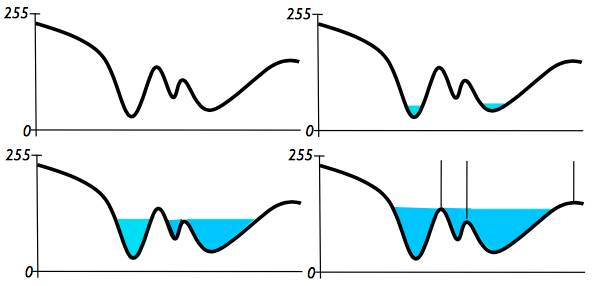
\includegraphics[width=0.6\columnwidth]{img/abordagem_flooding.jpg}
           \caption{\label{fig:abordagem_flooding}Abordagem "\textit{flooding based watershed}".\cite{regseg1}}
           % \vspace{2.0em}
       \end{center}
   \end{figure} 


A outra abordagem, denominada "\textit{rainfalling based watershed}" trata a imagem em níveis de cinza da mesma forma que a primeira, porém o fluxo de água ocorre a partir de gotas de água que ao incidirem em qualquer ponto da superfície escorrerão para um determinado vale, onde encontra-se um mínimo local. O conjunto de pontos para os quais a gota de água escorre para o mesmo local é interpretada como uma região e os limites entre duas regiões adjacentes,  interpretados como bordas, são as \textit{watersheds}.\citep{l6} 

% Figura 
	\begin{figure}[!htb]
       \begin{center}  
          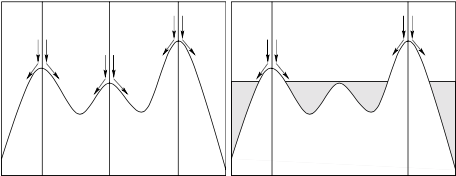
\includegraphics[width=0.6\columnwidth]{img/abordagem_rainfalling.jpg}
           \caption{\label{fig:abordagem_rainfalling}Abordagem "\textit{rainfalling based watershed}".\cite{ruparelia2012implementation}}
           % \vspace{2.0em}
       \end{center}
   \end{figure} 
	

Ambas abordagens tratam da mesma ideia básica por trás da técnica, sendo duas formas diferentes de ilustrar seus funcionamento sobre os quais diferentes algoritmos são propostos.

Um dos principais problemas relacionados à abordagem tradicional do \textit{watershed} é o problema de \textit{over-segmentation}. Para reduzir esse problema, diversas variações de algoritmos baseados na técnica de \textit{watershed} foram implementados, tal qual o algoritmo utilizado nessa pesquisa que será explicado detalhadamente na seção \ref{sec:alg} do capítulo \ref{cap:algoritmo}. Assim as diferenças entre o algoritmo proposto e o tradicional, como o implementado na biblioteca OpenCV, apresentada na seção \ref{sec:opencv} do capítulo \ref{cap:ferramentas}, conduzirão a uma análise comparativa entre os resultados obtidos por meio de cada um deles.

\section{\textit{Watershed Algorithm Based On Connected Components}}
Destacam-se as seguintes características entre este algoritmo e a abordagem tradicional \textit{watershed} que demonstram sua maior eficiência:

% \section{Características}
\begin{itemize}
    \item Fila FIFO ao invés de fila hierárquica - algoritmo tradicional - que requer sequências de acesso à memória não uniformes;
    \item Estrutura de dados mais simples; e
    \item Menor tempo de execução.
\end{itemize}    

Este algoritmo tem como princípio conectar cada \textit{pixel} (componente), caso este não seja o mínimo local, ao menor \textit{pixel} vizinho. Todos os \textit{pixels} direcionados para o mesmo mínimo local formam um segmento e são, portanto, rotulados da mesma forma.

% Figura
	\begin{figure}[!htb]
       \begin{center}  
          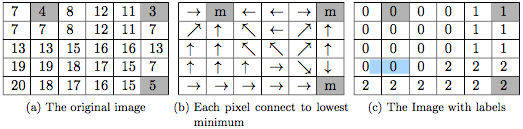
\includegraphics[width=0.9\columnwidth]{img/connected_components.jpg}
           \caption{\label{fig:connected_components}Ilustração do funcionamento da técnica \textit{Watershed Based On Connected Components}.\cite{ruparelia2012implementation}}
           % \vspace{2.0em}
       \end{center}
   \end{figure}

\section{Implementação do Algoritmo}\label{sec:alg}

O algoritmo de segmentação proposto nessa pesquisa, assim como os demais algoritmos baseados na técnica de segmentação por \textit{watershed}, segue a estrutura apresentada na Figura \ref{fig:diagrama_blocos_algoritmo}. A imagem original passa por uma etapa de pré-processamento, em que diferentes procedimentos são realizados. Após a etapa de pré-processamento, a imagem é segmentada pela técnica \textit{watershed} e seu resultado pode ser processado, na etapa de pós-processamento, a fim de corrigir algumas falhas geradas pelo processo de segmentação para, finalmente, obter a segmentação como resultado final.
Todas as etapas serão explicadas nas próximas seções de acordo como foram implementadas no algoritmo proposto por essa pesquisa.

% Figura
	\begin{figure}[!htb]
       \begin{center}  
          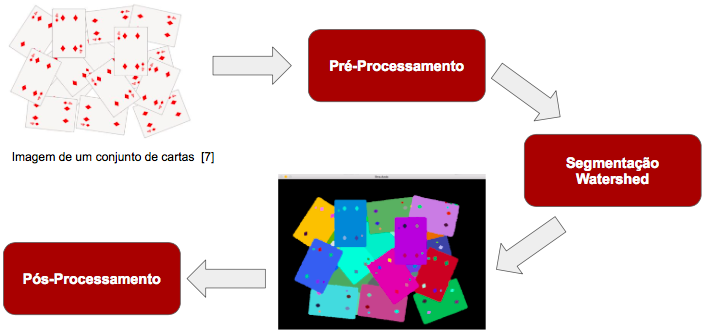
\includegraphics[width=0.7\columnwidth]{img/diagrama_blocos_algoritmo.jpg}
           \caption{\label{fig:diagrama_blocos_algoritmo}Diagrama de blocos do algoritmo de segmentação dessa pesquisa.}
           % \vspace{2.0em}
       \end{center}
   \end{figure} 

\subsection{Pré-Processamento}
A etapa de pré-processamento tem como objetivo preparar a imagem que será utilizada na segmentação efetivamente. Para isso alguns procedimentos são realizados com o objetivo de retirar ruídos e realçar bordas para facilitar o processo de segmentação a fim de obter um resultado mais eficiente. Além disso, assim como a etapa de pós-processamento, esta etapa visa diminuir o problema de \textit{over-segmentation}, o qual tende a ocorrer quando aplica-se a técnica de \textit{watershed}.
A ordem em que esses procedimentos ocorrem nesta etapa consta na estrutura apresentada pela Figura \ref{fig:diagrama_blocos_preprocessamento}.

% Figura
	\begin{figure}[!htb]
       \begin{center}  
          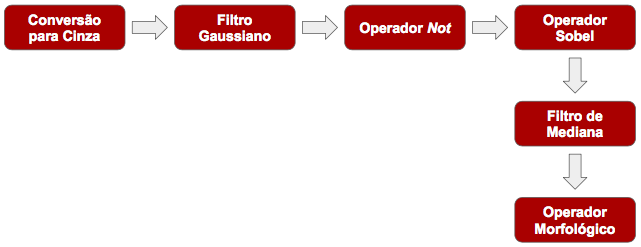
\includegraphics[width=0.8\columnwidth]{img/diagrama_blocos_preprocessamento.jpg}
           \caption{\label{fig:diagrama_blocos_preprocessamento}Diagrama de blocos da etapa de pré-processamento.}
           % \vspace{2.0em}
       \end{center}
   \end{figure}

\subsection*{Conversão para Cinza}
Um dos procedimentos realizados na etapa de pré-processamento é a conversão da imagem original colorida para a imagem em níveis de cinza. Utiliza-se a quantização em 256 níveis de cinza (8 bits), onde o nível zero representa o preto e o nível 255, o branco.
O objetivo dessa conversão é tratar a imagem em um canal já que o escopo da presente pesquisa é tratar imagens em escala de cinza.

\subsection*{Filtro Gaussiano}
O filtro gaussiano é utilizado como um dos primeiros procedimentos da etapa de pré-processamento a fim de remover os ruídos presentes na imagem a ser segmentada.


\subsection*{Operador \textit{Not}}
O operador not é utilizado no pré-processamento para que o algoritmo \textit{watersheed } seja executado da maneira correta, isto é, dos plateaus para os mínimos locais através. Ele inverte cada bit de um \textit{array}.

\subsection*{Operador Sobel}
Operador de detecção de bordas, que se baseia no operador gradiente. Esse operador é utilizado sobre a imagem resultante do operador \textit{not} com a finalidade de gerar uma imagem com as bordas detectadas brilhantes em um fundo (\textit{background}) mais escuro.

Computa-se os gradientes horizontal, \textit{Gx}, e vertical, \textit{Gy}, considerando uma janela de tamanho 3, isto é, \textit{3 x 3 pixels}, e calcula-se uma aproximação do gradiente em cada ponto da seguinte forma: \citep{sobel}

% Equação
\[G = |G_{x}| + |G_{y}|\]

% Código


\subsection*{Filtro de Mediana}
O objetivo do filtro de mediana é a redução ou, até mesmo, a remoção de ruídos das imagens, a fim de suavizá-las e torná-las mais tratáveis para o processo de segmentação. O filtro de mediana é eficaz para o tratamento de ruídos impulsivos, como o ruído Gaussiano (aleatório) e, principalmente, o ruído sal e pimenta, em que os \textit{pixels} ruidosos assumem os valores máximos e mínimos da imagem.
Para a implementação do filtro de mediana, considera-se uma imagem com \textit{n x m pixels} e um filtro com janela de \textit{k x k pixels}, onde \textit{k < n e k < m}. Em casa janela considerada na imagem, o valor de cada \textit{pixel} é substituído pelo valor da mediana da mesma janela. No algoritmo, usa-se \textit{k = 3} e o funcionamento do filtro pode ser entendido na Figura \ref{fig:filtromediana}.

% Figura
	\begin{figure}[!htb]
       \begin{center}  
          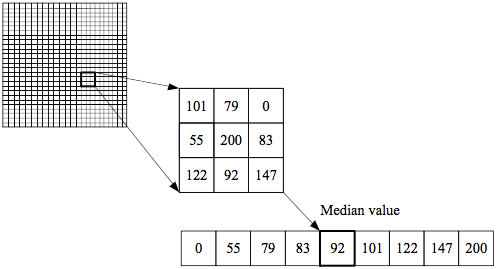
\includegraphics[width=0.8\columnwidth]{img/filtromediana.jpg}
           \caption{\label{fig:filtromediana}Ilustração do funcionamento do filtro de mediana.\cite{ruparelia2012implementation}}
           % \vspace{2.0em}
       \end{center}
   \end{figure}
   
% Código

\subsection*{Operadores Morfológicos}
Após a aplicação de um detector de bordas (operador Sobel) pode acontecer da imagem ficar com bordas "falhadas". Como a técnica de \textit{watershed} requer que as regiões estejam "fechadas", ou seja, sem falhas nas bordas, é aplicado um conjunto de operações morfológicas para conectar estas regiões fragmentadas. 
Existem duas operações morfológicas básicas:
% \section{Operações morfológicas básicas}
\begin{itemize}
    \item Erosão; e
    \item Dilatação.
\end{itemize}    

A biblioteca OpenCV fornece 5 transformações morfológicas baseadas nessas duas operações básicas:
% \section{Transformações morfológicas}
\begin{itemize}
    \item \textit{Opening};
    \item \textit{Closing};
    \item \textit{Morphological Gradient};
    \item \textit{Top Hat}; e 
    \item \textit{Black Hat}.
\end{itemize} 

No algoritmo utiliza-se apenas a transformação \textit{closing}, a qual é útil para o fechamento de bordas, removendo pequenos buracos que possam ter sido gerados nos procedimentos anteriores. \citep{morphology_transformations}

% Equação
\[dst = close(src, element) = erode(dilate(src, element))\]


\subsection{Segmentação por Técnica Baseada em \textit{Watershed}}
Dentre as duas principais abordagens da técnica de \textit{watershed} mencionadas na seção \ref{sec:watershed} do capítulo \ref{cap:algoritmo}, optou-se pela abordagem "\textit{rainfalling based watershed}" a fim de servir como base para a implementação da etapa de segmentação implementada neste algoritmo. Essa etapa é composta por três passos (\textit{steps}). 

\subsection{\textit{Step} 1}
% Explicar 
O objetivo do passo 1 é encontrar os mínimos locais na imagem. Inicialmente, o \textit{array} v[p] e percorre-se a imagem de cima à esquerda até abaixo à direita e, v[p] assumirá o valor zero se o valor de seu vizinho for menos ou igual ao seu, e o valor 1 caso contrário.


% Código 
\begin{algorithm}[H]
\SetAlgoLined

    \SetKwInOut{Input}{Input}
    \SetKwInOut{Output}{Output}

    \underline{STEP1} $(p)$\;
		\If{v[p] != 1}{
  		\For{cada n vizinho de p}{
   		\If{f[n] < f(p)}{
	   		v[p] = 1\;   		
   		}
   }
   }
 
\caption{Pseudo código para o passo um do algoritmo de \textit{watershed}. \cite{ruparelia2012implementation}}
\end{algorithm}




\subsection{\textit{Step} 2} 
% Explicar 
O fundamento do passo 2 é o de que se um \textit{pixel} está no \textit{plateau} e seu vizinho apontado para um dos mínimos locais, então o \textit{pixel} aponta para o respectivo vizinho. Para isso, considera-se os \textit{pixels} com v[p] diferente de 1 e com seus \textit{pixels} vizinhos no mesmo \textit{plateau} com v[p]=1, ou seja, regiões que não são de mínimo local. Em seguida, calcula-se a menor distancia até um mínimo local.

% Código 
\begin{algorithm}[H]
\SetAlgoLined

    \SetKwInOut{Input}{Input}
    \SetKwInOut{Output}{Output}

    \underline{STEP2} $(p)$\;
		
		  \If{v[p] != 1}{
  		min = VMAX, para cada n de p\\				
   		\If{f(n) = f(p) {\bf and} v[n] > 0 {\bf and} v[n] < min}{
	   		min = v[n]\;   		
   		}
   		\If{min != VMAX {\bf and} v[p] != (min+1)  }{
	   		v[p] = min+1\;   		
   		}
   
   }
 
\caption{Pseudo código para o passo dois do algoritmo de \textit{watershed}. \cite{ruparelia2012implementation}}
\end{algorithm}


\subsection{\textit{Step} 3}
% Explicar
O objetivo da da terceira etapa do algoritmo é separar os \textit{pixels} em regiões. Para isso, inicializa-se todos os \textit{pixels} com valor zero. Inicialmente, começa-se a definir as regiões a partir dos mínimos locais cujo v[p]=0 cujos \textit{pixels} vizinhos com o mesmo valor na escala de cinza ainda não estão associados a uma região definida. Essas regiões são propagadas para seus \textit{pixels} vizinhos de acordo com o valor de v[p] para criar regiões cujo centro é um mínimo local. Em seguida, regiões similares são criadas para todos os mínimos locais por este mesmo procedimento.

% Código 
\begin{algorithm}[H]
\SetAlgoLined

    \SetKwInOut{Input}{Input}
    \SetKwInOut{Output}{Output}

    \underline{STEP3} $(p)$\;
		
		lmin=LMAX, fmin=f(p)\\
   \uIf{v[p] = 0}{
        \For{cada n vizinho de p}{
            \If{f(n) = f(p) {\bf and} l[n] > 0  {\bf and} l[n] < lmin}{
                lmin = l[n]
            }
            \If{lmin = LMAX  {\bf and} l[p] = 0 }{
                lmin = New\_label+1
            }
        }
    }
    
    \uElseIf{v[p] = 1}{
       \For{cada n vizinho de p}{
            \If{f(n) < fmin}{
                fmin = f[n]
            }
        }
        \For{cada n vizinho de p}{
            \If{f(n) = fmin {\bf and} l[n] > 0 {\bf and} l[n] < lmin}{
                lmin = l[n]
            }
        }
       
    }   
    \Else{
        \For{cada n vizinho de p}{
            \If{f(n) = f(p) {\bf and} v[n] = v[p]-1 {\bf and} l[n] > 0 {\bf and} l[n] < lmin}{
                lmin = l[n]
            }
        } 
    }
    
    \If{lmin != LMAX {\bf and} l[n] != LMIN}{
        l[p] = lmin
    }
 
 
\caption{Pseudo código para o passo três do algoritmo de \textit{watershed}.\cite{ruparelia2012implementation}}
\end{algorithm}




\subsection{Pós-Processamento}
Após as etapas de pré-processamento e segmentação, ainda podem ser necessárias algumas correções relacionadas ao problema de \textit{over-segmentation}. É comum que tenhamos diferentes segmentos que fazem parte de uma mesma região. Para tanto pode-se utilizar algum método de  agrupamento para mesclar esses segmentos a fim de melhorar a qualidade da segmentação.